\documentclass[12pt,a4paper]{article}

% ---بسته‌های مورد نیاز---
\usepackage{geometry}
\usepackage{xcolor}
\usepackage{amsmath}
\usepackage{amsfonts}
\usepackage{graphicx}
\usepackage{tikz}
\usetikzlibrary{arrows.meta, shapes}
\usepackage{booktabs}
\usepackage{fancyhdr}
\usepackage{titlesec}
\usepackage{tcolorbox}
\usepackage{hyperref}
\usepackage{listings}
\usepackage{amssymb} % For checkmark symbol
\usepackage{pgfplots}
\pgfplotsset{compat=1.18}


% ---بسته زی‌پرشین برای نوشتار فارسی---
% این بسته باید تقریباً آخر از همه فراخوانی شود
\usepackage{xepersian}
\settextfont[Path="./", Extension=".ttf"]{XB-Niloofar}
\setdigitfont[Path="./", Extension=".ttf"]{XB-Niloofar}

% ---تنظیمات صفحه---
\geometry{
	a4paper,
	top=2.5cm,
	bottom=2.5cm,
	left=2.5cm,
	right=2.5cm
}
\setlength{\headheight}{16pt}

% ---تعریف رنگ‌ها---
\definecolor{codegreen}{rgb}{0,0.6,0}
\definecolor{codegray}{rgb}{0.5,0.5,0.5}
\definecolor{codepurple}{rgb}{0.58,0,0.82}
\definecolor{backcolour}{rgb}{0.95,0.95,0.92}
\definecolor{sectioncolor}{rgb}{0.0, 0.4, 0.6}
\definecolor{boxbackcolor}{rgb}{0.94, 0.97, 1.0}
\definecolor{darkblue}{rgb}{0.0, 0.0, 0.55}
\definecolor{darkred}{rgb}{0.55, 0.0, 0.0}

% ---سربرگ و پاورقی---
\pagestyle{fancy}
\fancyhf{}
\fancyhead[R]{\lr{Support Vector Machine (SVM)}}
\fancyhead[L]{مقدمه‌ای بر ماشین بردار پشتیبان}
\fancyfoot[C]{\thepage}

% ---شخصی‌سازی ظاهر بخش‌ها---
\titleformat{\section}
{\color{sectioncolor}\Large\bfseries}
{\thesection}{1em}{}
\titleformat{\subsection}
{\color{sectioncolor}\large\bfseries}
{\thesubsection}{1em}{}
\titleformat{\subsubsection}
{\color{sectioncolor}\normalsize\bfseries}
{\thesubsubsection}{1em}{}

% ---تنظیمات هایپرلینک---
\hypersetup{
	colorlinks=true,
	linkcolor=darkblue,
	citecolor=darkred,
	urlcolor=blue,
	pdfpagemode=FullScreen,
	unicode=true
}

% ---جعبه‌های رنگی برای تعاریف و فرمول‌ها---
\newtcolorbox{infobox}[1][]{
	colback=boxbackcolor,
	colframe=sectioncolor,
	fonttitle=\bfseries,
	arc=3mm,
	#1
}

\title{
	\begin{center}
		{\Huge \bfseries مقدمه‌ای بر روش ماشین بردار پشتیبان (SVM)} \\
		\vspace{1cm}
		{\large یک راهنمای ساده و جامع برای پژوهشگران علوم اعصاب}
	\end{center}
}
\author{\href{https://github.com/MohammadMahdi-Sharifbeigy}{محمدمهدی شریف بیگی} \\ 
	\lr{MohammadMahdi Sharifbeigy}}
\date{\today}

\begin{document}
	
	\maketitle
	\thispagestyle{empty}
	\newpage
	
	\tableofcontents
	\thispagestyle{empty}
	\newpage
	
	\section{ماشین بردار پشتیبان (SVM) چیست؟}
	\label{sec:intro}
	
	ماشین بردار پشتیبان یا \lr{(Support Vector Machine - SVM)} یکی از قدرتمندترین و پرکاربردترین الگوریتم‌های یادگیری ماشین با نظارت \lr{(Supervised Learning)} است که عمدتاً برای مسائل طبقه‌بندی \lr{(Classification)} و همچنین رگرسیون \lr{(Regression)} به کار می‌رود. ایده اصلی \lr{SVM} بسیار هوشمندانه و در عین حال ساده است: پیدا کردن یک خط یا یک صفحه (که به آن \textbf{اَبَرصفحه} یا \lr{Hyperplane} می‌گوییم) که به بهترین شکل ممکن داده‌های مربوط به کلاس‌های مختلف را از یکدیگر جدا کند.
	
	«بهترین شکل ممکن» در اینجا به معنای پیدا کردن ابرصفحه‌ای است که بیشترین فاصله را با نزدیک‌ترین نمونه‌های هر کلاس داشته باشد. این فاصله، \textbf{حاشیه} \lr{(Margin)} نامیده می‌شود. \lr{SVM} با بیشینه‌سازی این حاشیه، یک مرز تصمیم‌گیری قدرتمند و قابل تعمیم ایجاد می‌کند که در مقابل نویز و داده‌های جدید عملکرد خوبی از خود نشان می‌دهد.
	
	در حوزه علوم اعصاب و تحلیل سیگنال‌های الکتروفیزیولوژی، از \lr{SVM} می‌توان برای کاربردهای متنوعی استفاده کرد، مانند:
	\begin{itemize}
		\item \textbf{واسط‌های مغز و کامپیوتر \lr{(BCI)}:} تشخیص و طبقه‌بندی الگوهای مغزی مرتبط با تصور حرکات مختلف (مثلاً حرکت دست راست در مقابل دست چپ).
		\item \textbf{تشخیص بیماری:} تفکیک سیگنال‌های \lr{EEG} افراد سالم از بیماران مبتلا به صرع یا آلزایمر.
		\item \textbf{تحلیل حالت‌های شناختی:} طبقه‌بندی وضعیت‌های ذهنی مختلف مانند تمرکز، آرامش یا خواب‌آلودگی بر اساس ویژگی‌های استخراج‌شده از سیگنال‌های مغزی.
	\end{itemize}
	
	\section{جداکننده خطی و مفهوم حاشیه بیشینه}
	\label{sec:max_margin}
	
	بیایید با یک مثال ساده شروع کنیم. فرض کنید داده‌های ما در یک فضای دو بعدی قرار دارند و به دو کلاس مختلف (مثلاً دایره‌های آبی و مربع‌های قرمز) تعلق دارند. هدف ما پیدا کردن یک خط است که این دو کلاس را از هم جدا کند.
	
	\begin{figure}[h!]
		\centering
		\begin{tikzpicture}[scale=1.2]
			% Data points
			\foreach \x/\y in {1/1.5, 1.5/2.5, 2/2, 2.5/3}
			\fill[blue] (\x,\y) circle (2.5pt);
			\foreach \x/\y in {3.5/1, 4/1.8, 4.5/0.8, 5/1.5}
			\fill[red] (\x,\y) rectangle ++(0.15,0.15);
			
			% Hyperplanes
			\draw[gray, dashed, thick] (0.5, 4) -- (5.5, 0) node[right, black, scale=0.8] {\rl{جداکننده ۱}};
			\draw[gray, dotted, thick] (1, 0) -- (4, 4) node[right, black, scale=0.8] {\rl{جداکننده ۲}};
			\draw[darkblue, thick, -] (0, 1.5) -- (6, 3) node[above, black, scale=0.8] {\textbf{\rl{جداکننده بهینه}}};
			
		\end{tikzpicture}
		\caption{چندین خط می‌توانند دو کلاس را از هم جدا کنند، اما کدام یک بهترین است؟}
		\label{fig:hyperplanes}
	\end{figure}
	
	همانطور که در شکل \ref{fig:hyperplanes} می‌بینید، بی‌نهایت خط می‌توان برای جداسازی این دو کلاس رسم کرد. اما \lr{SVM} به دنبال خطی است که بیشترین «فضای خالی» یا «حاشیه امن» را بین خود و نزدیک‌ترین نقاط هر دو کلاس ایجاد کند. این خط را \textbf{اَبَرصفحه با حاشیه بیشینه} \lr{(Maximal Margin Hyperplane)} می‌نامیم.
	
	\begin{figure}[h!]
		\centering
		\begin{tikzpicture}[scale=1.3]
			% Data points
			% Blue class
			\node[circle, fill=blue, inner sep=2pt] (p1) at (1, 0.5) {};
			\node[circle, fill=blue, inner sep=2pt] (p2) at (2, 0) {};
			% Blue SV on the margin y=0.5x
			\node[circle, fill=blue, inner sep=2pt, label=below:{\lr{\textbf{SV}}}] (p3) at (3, 1.5) {};
			
			% Red class
			\node[draw, fill=red, inner sep=2pt, shape=rectangle] (p4) at (3, 5) {};
			\node[draw, fill=red, inner sep=2pt, shape=rectangle] (p6) at (4, 4) {};
			% Red SV on the margin y=0.5x+2
			\node[draw, fill=red, inner sep=2pt, shape=rectangle, label=above:{\lr{\textbf{SV}}}] (p5) at (2, 3) {};
			
			% Hyperplane and margins (recalculated for accuracy)
			% Hyperplane y = 0.5x + 1
			\draw[darkblue, thick] (0, 1) -- (6, 4) node[pos=0.9, sloped, above] {\rl{ابرصفحه: $\mathbf{w}^T \mathbf{x} + b = 0$}};
			% Upper Margin y = 0.5x + 2
			\draw[darkblue, dashed, thick] (0, 2) -- (6, 5) node[pos=0.9, sloped, above] {$\mathbf{w}^T \mathbf{x} + b = 1$};
			% Lower Margin y = 0.5x
			\draw[darkblue, dashed, thick] (0, 0) -- (6, 3) node[pos=0.9, sloped, below] {$\mathbf{w}^T \mathbf{x} + b = -1$};
			
			% Margin arrow
			\draw[{Latex}-{Latex}, thick] (3, 1.5) -- (2.2, 3.1);
			\node[anchor=south west] at (2.6, 2.3) {حاشیه};
			
			\node at (0.5,3) {\rl{کلاس ۱+}};
			\node at (5.5,1.5) {\rl{کلاس ۱-}};
		\end{tikzpicture}
		\caption{ابرصفحه با حاشیه بیشینه. نقاطی که روی خطوط حاشیه قرار دارند، \textbf{بردارهای پشتیبان} \lr{(Support Vectors)} نامیده می‌شوند.}
		\label{fig:max_margin}
	\end{figure}
	
	ابرصفحه به صورت ریاضی با معادله $f(\mathbf{x}) = \mathbf{w}^T \mathbf{x} + b = 0$ تعریف می‌شود، که در آن:
	\begin{itemize}
		\item $\mathbf{w}$ یک بردار عمود بر ابرصفحه است (بردار وزن‌ها). جهت این بردار، جهت جداسازی را نشان می‌دهد.
		\item $\mathbf{x}$ بردار ویژگی‌های یک نقطه داده است.
		\item $b$ یک مقدار بایاس است که موقعیت ابرصفحه را نسبت به مبدأ مختصات مشخص می‌کند.
	\end{itemize}
	دو خط موازی دیگر که حاشیه را تعریف می‌کنند، با معادلات $\mathbf{w}^T \mathbf{x} + b = 1$ و $\mathbf{w}^T \mathbf{x} + b = -1$ مشخص می‌شوند. فاصله بین این دو خط برابر با $\frac{2}{||\mathbf{w}||}$ است. هدف SVM بیشینه‌سازی این فاصله است که معادل با کمینه‌سازی $||\mathbf{w}||$ (یا به طور معادل $\frac{1}{2}||\mathbf{w}||^2$ برای سادگی محاسبات) می‌باشد.
	
	\begin{infobox}[title={مسئله بهینه‌سازی (حاشیه سخت)}]
		\begin{latin}
			\begin{equation}
				\underset{\mathbf{w}, b}{\text{minimize}} \quad \frac{1}{2} ||\mathbf{w}||^2
			\end{equation}
			\begin{equation}
				\text{subject to} \quad y_i(\mathbf{w}^T \mathbf{x}_i + b) \geq 1, \quad \forall i=1, \dots, n
			\end{equation}
		\end{latin}
		که در آن $y_i$ برچسب کلاس نمونه $i$-ام است (با مقدار ۱+ یا ۱-). قید (۲) تضمین می‌کند که تمام نقاط داده به درستی و خارج از حاشیه طبقه‌بندی شوند.
	\end{infobox}
	
	\section{مقابله با داده‌های جداناپذیر: حاشیه نرم}
	\label{sec:soft_margin}
	
	مدل «حاشیه سخت» \lr{(Hard Margin)} تنها زمانی کار می‌کند که داده‌ها کاملاً به صورت خطی جداپذیر باشند. اما در دنیای واقعی، داده‌ها اغلب دارای نویز هستند یا با یکدیگر همپوشانی دارند. راه حل این مشکل، استفاده از \textbf{حاشیه نرم} \lr{(Soft Margin)} است. در این روش، به مدل اجازه می‌دهیم که برخی از نقاط را به اشتباه طبقه‌بندی کند یا آن‌ها را درون حاشیه قرار دهد. برای هر نقطه، یک \textbf{متغیر کُندی} \lr{(Slack Variable)} با نماد $\xi_i \geq 0$ تعریف می‌کنیم.
	
	\begin{figure}[h!]
		\centering
		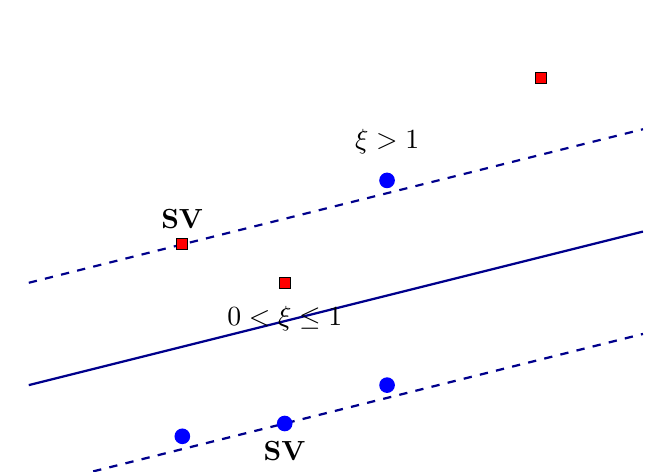
\begin{tikzpicture}[scale=1.3]
			% Hyperplane and margins
			\draw[darkblue, thick] (0, 1.5) -- (6, 3);
			\draw[darkblue, dashed, thick] (0, 2.5) -- (6, 4);
			\draw[darkblue, dashed, thick] (0, 0.5) -- (6, 2);
			
			% Data points
			% Blue class (class -1)
			\node[circle, fill=blue, inner sep=2pt] at (1.5, 1) {};
			\node[circle, fill=blue, inner sep=2pt] at (3.5, 1.5) {};
			% Blue SV on the margin
			\node[circle, fill=blue, inner sep=2pt, label=below:{\lr{\textbf{SV}}}] at (2.5, 1.125) {};
			% Misclassified blue point (xi > 1)
			\node[circle, fill=blue, inner sep=2pt, label={[align=center, label distance=1mm]above:{\lr{$\xi > 1$}}} ] at (3.5, 3.5) {};
			
			% Red class (class +1)
			\node[draw, fill=red, inner sep=2pt, shape=rectangle] at (5, 4.5) {};
			% Red SV on the margin
			\node[draw, fill=red, inner sep=2pt, shape=rectangle, label=above:{\lr{\textbf{SV}}}] at (1.5, 2.875) {};
			% Red point inside margin (0 < xi <= 1)
			\node[draw, fill=red, inner sep=2pt, shape=rectangle, label={[align=center, label distance=1mm]below:{\lr{$0 < \xi \le 1$}}} ] at (2.5, 2.5) {};
			
		\end{tikzpicture}
		\caption{در روش حاشیه نرم، به برخی نقاط اجازه داده می‌شود که حاشیه را نقض کنند (\lr{$\xi_i > 0$}). این نقاط متخلف نیز بردار پشتیبان محسوب می‌شوند.}
		\label{fig:soft_margin}
	\end{figure}
	
	مسئله بهینه‌سازی به شکل زیر تغییر می‌کند:
	\begin{infobox}[title={مسئله بهینه‌سازی (حاشیه نرم)}]
		\begin{latin}
			\begin{equation}
				\underset{\mathbf{w}, b, \boldsymbol{\xi}}{\text{minimize}} \quad \frac{1}{2} ||\mathbf{w}||^2 + C \sum_{i=1}^{n} \xi_i
			\end{equation}
			\begin{equation}
				\text{subject to} \quad y_i(\mathbf{w}^T \mathbf{x}_i + b) \geq 1 - \xi_i, \quad \text{and} \quad \xi_i \geq 0, \quad \forall i
			\end{equation}
		\end{latin}
		در اینجا پارامتر جدید $C > 0$ \textbf{پارامتر تنظیم} یا \lr{Regularization Parameter} نام دارد. این پارامتر یک توازن \lr{(Trade-off)} بین دو هدف متضاد برقرار می‌کند:
		\begin{itemize}
			\item \textbf{بیشینه‌سازی حاشیه:} که با کمینه کردن جمله $\frac{1}{2} ||\mathbf{w}||^2$ (مدل ساده) به دست می‌آید.
			\item \textbf{کمینه‌سازی خطای طبقه‌بندی:} که با کمینه کردن جمله $\sum \xi_i$ (دقت بالا روی داده‌های آموزش) حاصل می‌شود.
		\end{itemize}
		مقدار بزرگ $C$ به معنای جریمه سنگین برای خطاها است و مدل را به سمت یک حاشیه باریک‌تر با خطای کمتر سوق می‌دهد (ریسک بیش‌برازش یا \lr{Overfitting}). مقدار کوچک $C$ به مدل اجازه می‌دهد حاشیه پهن‌تری داشته باشد، حتی اگر به قیمت چند خطای طبقه‌بندی بیشتر تمام شود (ریسک کم‌برازش یا \lr{Underfitting}).
	\end{infobox}
	
	\subsection{تابع هزینه Hinge Loss}
	می‌توان فرمول‌بندی حاشیه نرم را از دیدگاه دیگری نیز مشاهده کرد: با استفاده از یک \textbf{تابع هزینه} \lr{(Loss Function)}. تابع هزینه‌ای که SVM از آن استفاده می‌کند \textbf{Hinge Loss} نام دارد و به صورت زیر تعریف می‌شود:
	\begin{infobox}[title={تابع هزینه Hinge Loss}]
		\begin{equation}
			L(y_i, f(\mathbf{x}_i)) = \max(0, 1 - y_i f(\mathbf{x}_i))
		\end{equation}
		که در آن $f(\mathbf{x}_i) = \mathbf{w}^T \mathbf{x}_i + b$ خروجی مدل است. این تابع هزینه دارای ویژگی‌های زیر است:
		\begin{itemize}
			\item اگر یک نمونه به درستی و خارج از حاشیه طبقه‌بندی شود ($y_i f(\mathbf{x}_i) \ge 1$)، هزینه آن صفر است.
			\item اگر یک نمونه درون حاشیه قرار گیرد یا به اشتباه طبقه‌بندی شود ($y_i f(\mathbf{x}_i) < 1$)، هزینه آن به صورت خطی با فاصله از مرز حاشیه افزایش می‌یابد.
		\end{itemize}
		در واقع، متغیرهای کُندی $\xi_i$ دقیقاً برابر با مقدار \lr{Hinge Loss} برای هر نمونه هستند: 
		
		$\xi_i = \max(0, 1 - y_i f(\mathbf{x}_i))$. بنابراین، مسئله بهینه‌سازی حاشیه نرم را می‌توان به صورت زیر نیز نوشت که به آن \textbf{فرمول‌بندی اولیه نامقید} می‌گویند:
		\begin{equation}
			\underset{\mathbf{w}, b}{\text{minimize}} \quad \frac{1}{2} ||\mathbf{w}||^2 + C \sum_{i=1}^{n} \max(0, 1 - y_i(\mathbf{w}^T \mathbf{x}_i + b))
		\end{equation}
	\end{infobox}
	
	\section{ریاضیات بهینه‌سازی: لاگرانژ، دوگانگی و KKT}
	\label{sec:math}
	مسئله بهینه‌سازی SVM یک مسئله \textbf{برنامه‌نویسی درجه دوم} \lr{(Quadratic Programming - QP)} است. برای حل این مسئله، از روش قدرتمند \textbf{مضارب لاگرانژ} استفاده می‌کنیم. تابع \textbf{لاگرانژین} اولیه به صورت زیر تعریف می‌شود:
	\begin{latin}
		\begin{equation}
			L_P(\mathbf{w}, b, \boldsymbol{\xi}, \boldsymbol{\alpha}, \boldsymbol{\mu}) = \frac{1}{2}||\mathbf{w}||^2 + C\sum\xi_i - \sum\alpha_i[y_i(\mathbf{w}^T\mathbf{x}_i + b) - 1 + \xi_i] - \sum\mu_i\xi_i
		\end{equation}
	\end{latin}
	که در آن $\alpha_i \ge 0$ و $\mu_i \ge 0$ مضارب لاگرانژ هستند. با مشتق‌گیری و ساده‌سازی، به \textbf{مسئله دوگان} \lr{(Dual Problem)} می‌رسیم:
	\begin{infobox}[title={مسئله بهینه‌سازی دوگان}]
		\begin{latin}
			\begin{equation}
				\underset{\boldsymbol{\alpha}}{\text{maximize}} \quad W(\boldsymbol{\alpha}) = \sum_{i=1}^{n} \alpha_i - \frac{1}{2} \sum_{i=1}^{n} \sum_{j=1}^{n} \alpha_i \alpha_j y_i y_j (\mathbf{x}_i^T \mathbf{x}_j)
			\end{equation}
			\begin{equation}
				\text{subject to} \quad \sum_{i=1}^{n} \alpha_i y_i = 0, \quad \text{and} \quad 0 \le \alpha_i \le C, \quad \forall i
			\end{equation}
		\end{latin}
	\end{infobox}
	نکته کلیدی این است که مسئله دوگان فقط به متغیرهای $\alpha_i$ بستگی دارد و داده‌ها تنها از طریق ضرب داخلی $(\mathbf{x}_i^T \mathbf{x}_j)$ در آن ظاهر می‌شوند. این ویژگی اساس کار \textbf{ترفند کرنل} است.
	
	\subsection{شرایط کاروش-کوهن-تاکر (KKT)}
	شرایط \lr{Karush-Kuhn-Tucker (KKT)} ارتباط بین مسئله اولیه و دوگان را برقرار کرده و تفسیر جالبی از متغیرهای $\alpha_i$ ارائه می‌دهند:
	\begin{itemize}
		\item اگر $\alpha_i = 0$ باشد، نقطه $\mathbf{x}_i$ به درستی و خارج از حاشیه طبقه‌بندی شده است. این نقطه در تعیین مرز نقشی ندارد.
		\item اگر $0 < \alpha_i < C$ باشد، آنگاه $\xi_i = 0$ و نقطه $\mathbf{x}_i$ دقیقاً روی حاشیه قرار دارد. این نقطه یک \textbf{بردار پشتیبان} است.
		\item اگر $\alpha_i = C$ باشد، آنگاه $\xi_i > 0$ و نقطه $\mathbf{x}_i$ یا درون حاشیه قرار دارد یا به اشتباه طبقه‌بندی شده است. این نقطه نیز یک \textbf{بردار پشتیبان} است.
	\end{itemize}
	این ویژگی به این معناست که مرز تصمیم‌گیری تنها توسط زیرمجموعه کوچکی از داده‌ها (بردارهای پشتیبان) تعریف می‌شود.
	
	\section{ترفند کرنل: حرکت به ابعاد بالاتر}
	\label{sec:kernel}
	تا اینجا فرض کردیم که داده‌ها به صورت خطی جداپذیر هستند. اما اگر مرز بین کلاس‌ها یک منحنی پیچیده باشد، چه باید کرد؟
	\begin{figure}[h!]
		\centering
		\begin{tikzpicture}[scale=1]
			% Panel A: Non-linear data
			\begin{scope}[xshift=-4.5cm]
				\node at (2, 4) {(الف) \rl{داده‌های جداناپذیر خطی}};
				\foreach \i in {0, 30, ..., 330} \fill[blue] (\i:1.5) circle (2.5pt);
				\foreach \i in {15, 45, ..., 345} \fill[red] (\i:2.5) rectangle ++(0.15,0.15);
				\draw[->] (-3,0) -- (3,0) node[below] {$x_1$}; \draw[->] (0,-3) -- (0,3) node[left] {$x_2$};
			\end{scope}
			
			\draw[-{Stealth[length=5mm, width=3mm]}, line width=1.5pt] (-0.5, 1) -- (1, 1) node[midway, above] {\rl{نگاشت} $\phi$};
			
			% Panel B: Linearly separable in 3D
			\begin{scope}[xshift=3cm, yshift=0cm]
				\node at (0, 4) {(ب) \rl{داده‌های جداشده در فضای ویژگی}};
				\begin{axis}[yshift=-1.5cm,view={120}{30}, axis lines=center, xlabel={$x_1$}, ylabel={$x_2$}, zlabel={$x_1^2+x_2^2$}, xtick=\empty, ytick=\empty, ztick=\empty, width=7cm, height=6.5cm]
					\addplot3[surf, opacity=0.3, domain=-2:2, domain y=-2:2, samples=21, color=darkblue!50] {4};
					\addplot3[only marks, mark=*, blue, mark size=1.5pt] coordinates {(1.5,0,2.25) (1.3,0.75,2.25) (0.75,1.3,2.25) (0,1.5,2.25) (-0.75,1.3,2.25) (-1.3,0.75,2.25) (-1.5,0,2.25) (-1.3,-0.75,2.25) (-0.75,-1.3,2.25) (0,-1.5,2.25) (0.75,-1.3,2.25) (1.3,-0.75,2.25)};
					\addplot3[only marks, mark=square*, red, mark size=1.5pt] coordinates {(2.48,0.43,6.25) (1.77,1.77,6.25) (0.43,2.48,6.25) (-0.43,2.48,6.25) (-1.77,1.77,6.25) (-2.48,0.43,6.25) (-2.48,-0.43,6.25) (-1.77,-1.77,6.25) (-0.43,-2.48,6.25) (0.43,-2.48,6.25) (1.77,-1.77,6.25) (2.48,-0.43,6.25)};
				\end{axis}
			\end{scope}
		\end{tikzpicture}
		\caption{ایده اصلی ترفند کرنل: نگاشت داده‌ها به یک فضای با ابعاد بالاتر که در آن به صورت خطی جداپذیر شوند.}
		\label{fig:kernel_trick}
	\end{figure}
	
	ایده \textbf{ترفند کرنل} \lr{(Kernel Trick)} این است که به جای محاسبه پرهزینه نگاشت $ \phi(\mathbf{x}) $، مستقیماً ضرب داخلی $\phi(\mathbf{x}_i)^T \phi(\mathbf{x}_j)$ را با استفاده از یک تابع کرنل $K(\mathbf{x}_i, \mathbf{x}_j)$ محاسبه کنیم.
	\begin{infobox}[title={تابع کرنل و شرط مرسر}]
		\begin{equation}
			K(\mathbf{x}_i, \mathbf{x}_j) = \phi(\mathbf{x}_i)^T \phi(\mathbf{x}_j)
		\end{equation}
		یک تابع برای اینکه بتواند به عنوان یک کرنل معتبر استفاده شود، باید \textbf{شرط مرسر} را برآورده کند. این شرط تضمین می‌کند که ماتریس حاصل از اعمال کرنل بر روی تمام زوج داده‌ها، یک ماتریس نیمه معین مثبت \lr{(Positive Semi-definite)} باشد.
	\end{infobox}
	
	\subsection{انواع کرنل‌های متداول}
	\begin{itemize}
		\item \textbf{کرنل خطی:} $K(\mathbf{x}_i, \mathbf{x}_j) = \mathbf{x}_i^T \mathbf{x}_j$.
		\item \textbf{کرنل چندجمله‌ای:} $K(\mathbf{x}_i, \mathbf{x}_j) = (\gamma \mathbf{x}_i^T \mathbf{x}_j + r)^d$.
		\item \textbf{کرنل تابع پایه شعاعی (RBF):} $K(\mathbf{x}_i, \mathbf{x}_j) = \exp(-\gamma ||\mathbf{x}_i - \mathbf{x}_j||^2)$. این کرنل محبوب‌ترین انتخاب است.
		\item \textbf{کرنل کسینوسی:} $K(\mathbf{x}_i, \mathbf{x}_j) = \frac{\mathbf{x}_i^T \mathbf{x}_j}{||\mathbf{x}_i|| \cdot ||\mathbf{x}_j||}$.
	\end{itemize}
	
	\section{پرسش و پاسخ‌های عملی}
	\label{sec:faq}
	
	\subsection{چرا SVM به مقیاس‌بندی ویژگی‌ها حساس است؟}
	تابع هزینه SVM تلاش می‌کند تا فاصله‌ها را بیشینه کند. اگر یک ویژگی دارای مقیاس بسیار بزرگتری نسبت به بقیه باشد، فاصله در آن بُعد بر محاسبات غلبه خواهد کرد. به همین دلیل، \textbf{استانداردسازی} یا \textbf{نرمال‌سازی} داده‌ها قبل از آموزش SVM یک مرحله ضروری است.
	
	\subsection{SVM چگونه مسائل چندکلاسه را حل می‌کند؟}
	SVM ذاتاً یک طبقه‌بند دودویی است. برای حل مسائل با بیش از دو کلاس، از دو استراتژی رایج استفاده می‌شود:
	\begin{itemize}
		\item \textbf{یک در مقابل بقیه \lr{(One-vs-Rest - OvR)}:} برای $K$ کلاس، $K$ طبقه‌بند SVM آموزش داده می‌شود.
		\item \textbf{یک در مقابل یک \lr{(One-vs-One - OvO)}:} برای $K$ کلاس، تعداد $\frac{K(K-1)}{2}$ طبقه‌بند آموزش داده می‌شود. این روش معمولاً نتایج بهتری دارد اما از نظر محاسباتی سنگین‌تر است.
	\end{itemize}
	
	\subsection{تأثیر پارامترهای C و Gamma چگونه است؟}
	دو پارامتر $C$ و $\gamma$ (در کرنل RBF) نقش حیاتی در کنترل \textbf{توازن بایاس-واریانس} \lr{(Bias-Variance Trade-off)} دارند.
	\begin{itemize}
		\item \textbf{پارامتر $C$ (هزینه):} همانطور که قبلاً گفته شد، $C$ میزان جریمه برای طبقه‌بندی اشتباه را کنترل می‌کند. $C$ بالا به معنای جریمه سنگین (مدل پیچیده، واریانس بالا) و $C$ پایین به معنای جریمه سبک (مدل ساده، بایاس بالا) است.
		\item \textbf{پارامتر $\gamma$ (گاما):} این پارامتر در کرنل RBF، میزان تأثیر یک نمونه آموزشی را مشخص می‌کند. مقدار کم $\gamma$ به معنای تأثیر زیاد (شعاع بزرگ) است، که منجر به یک مرز تصمیم‌گیری نرم و کلی می‌شود (بایاس بالا). مقدار زیاد $\gamma$ به معنای تأثیر کم (شعاع کوچک) است، که باعث می‌شود مرز تصمیم‌گیری به شدت به نمونه‌های آموزشی نزدیک شود و پیچیده گردد (واریانس بالا و ریسک بیش‌برازش).
	\end{itemize}
	پیدا کردن ترکیب بهینه از این دو پارامتر معمولاً با روش‌هایی مانند جستجوی شبکه‌ای \lr{(Grid Search)} و اعتبارسنجی متقابل انجام می‌شود.
	
	\subsection{مقایسه فلسفه کرنل RBF و کرنل کسینوسی}
	این دو کرنل دو دیدگاه متفاوت برای سنجش «شباهت» بین نقاط دارند:
	\begin{itemize}
		\item \textbf{کرنل RBF (مبتنی بر فاصله):} این کرنل شباهت را بر اساس \textbf{نزدیکی} در فضای اقلیدسی می‌سنجد. مرزهای تصمیم آن \textbf{محلی و منحنی} هستند و خوشه‌های داده را احاطه می‌کنند. این کرنل به اندازه (magnitude) بردارها حساس است.
		\item \textbf{کرنل کسینوسی (مبتنی بر جهت):} این کرنل شباهت را بر اساس \textbf{زاویه} (جهت) بین بردارها نسبت به مبدأ مختصات می‌سنجد و اندازه بردارها را نادیده می‌گیرد. مرزهای تصمیم آن به صورت \textbf{خطوط صاف و شعاعی} هستند که از مبدأ سرچشمه می‌گیرند. این کرنل در حوزه‌هایی مانند پردازش متن که جهت بردار (کلمات کلیدی) مهم‌تر از طول آن (تعداد کلمات) است، کاربرد دارد.
	\end{itemize}
	
	\subsection{SVM در برابر نویز و داده‌های پرت چگونه عمل می‌کند؟}
	این سؤال مستقیماً به مفهوم \textbf{حاشیه نرم} و نقش پارامتر تنظیم $C$ بازمی‌گردد. مکانیزم اصلی SVM برای مقابله با نویز و داده‌های پرت، «نادیده گرفتن» هوشمندانه آن‌هاست.
	\begin{itemize}
		\item \textbf{داده پرت (Outlier):} یک داده پرت نقطه‌ای است که بسیار دور از سایر داده‌های کلاس خود قرار گرفته است. در مدل حاشیه سخت، تنها یک داده پرت می‌تواند موقعیت ابرصفحه را به کلی تغییر داده و حاشیه را بسیار باریک کند. اما در مدل حاشیه نرم، اگر هزینه طبقه‌بندی اشتباه آن نقطه (که توسط $C$ کنترل می‌شود) کمتر از هزینه کاهش شدید عرض حاشیه باشد، الگوریتم ترجیح می‌دهد آن نقطه را اشتباه طبقه‌بندی کند (یعنی $\xi_i > 0$) تا یک حاشیه پهن و سالم برای بقیه داده‌ها حفظ شود.
		\item \textbf{نویز (Noise):} نویز به نقاطی اطلاق می‌شود که در منطقه متعلق به کلاس دیگر ظاهر می‌شوند. SVM با حاشیه نرم به سادگی به این نقاط اجازه می‌دهد که در سمت اشتباه مرز قرار بگیرند (تبدیل به خطای طبقه‌بندی شوند) تا از ایجاد یک مرز تصمیم‌گیری بیش از حد پیچیده و پرپیچ‌وخم (بیش‌برازش) که سعی در جدا کردن تک‌تک نقاط دارد، جلوگیری کند.
	\end{itemize}
	به طور خلاصه، با تنظیم مناسب پارامتر $C$ (معمولاً با اعتبارسنجی متقابل)، SVM می‌تواند بین حفظ یک حاشیه بزرگ (که قدرت تعمیم را بالا می‌برد) و طبقه‌بندی صحیح تمام نقاط (که به نویز حساس است) تعادل برقرار کند و در نتیجه نسبت به داده‌های پرت مقاوم باشد.
	
	\subsection{نفرین ابعاد و بُعد VC چه هستند؟}
	این دو مفهوم نظری از حوزه یادگیری آماری به ما کمک می‌کنند تا بفهمیم چرا SVM با وجود قدرت بالایش، دچار بیش‌برازش نمی‌شود.
	
	\subsubsection{نفرین ابعاد (\lr{Curse of Dimensionality})}
	این اصطلاح به مشکلات متعددی اشاره دارد که هنگام کار با داده‌ها در فضاهای با ابعاد بسیار بالا رخ می‌دهد. با افزایش تعداد ویژگی‌ها (ابعاد)، حجم فضا به صورت نمایی افزایش می‌یابد. در نتیجه، داده‌ها به شدت پراکنده و دور از هم می‌شوند. این پراکندگی باعث می‌شود الگوریتم‌هایی که بر اساس فاصله یا همسایگی کار می‌کنند (مانند k-NN) کارایی خود را از دست بدهند، زیرا مفهوم «نزدیکی» بی‌معنا می‌شود.
	
	\textbf{SVM چگونه با این مشکل مقابله می‌کند؟} به طور شگفت‌انگیزی، SVM نه تنها از نفرین ابعاد رنج نمی‌برد، بلکه اغلب از آن سود می‌برد. دلیل این امر آن است که مرز تصمیم‌گیری در SVM تنها توسط \textbf{بردارهای پشتیبان} تعریف می‌شود، نه تمام داده‌ها. در یک فضای با ابعاد بالا، احتمال اینکه داده‌ها به صورت خطی جداپذیر شوند، بیشتر می‌شود. ترفند کرنل این ایده را به نهایت خود می‌رساند و داده‌ها را به یک فضای با ابعاد بسیار بالا (حتی بی‌نهایت) می‌برد تا یک ابرصفحه جداکننده پیدا کند، بدون آنکه هزینه محاسباتی این فضا را متحمل شود.
	
	\subsubsection{بُعد VC (\lr{Vapnik-Chervonenkis Dimension})}
	بُعد VC یک معیار برای سنجش \textbf{ظرفیت، پیچیدگی یا قدرت} یک مدل طبقه‌بندی است. به طور شهودی، بُعد VC برابر با بیشترین تعداد نقاطی است که مدل می‌تواند آن‌ها را به تمام ترکیبات ممکن برچسب‌گذاری کند (به اصطلاح \lr{shatter} کند).
	\begin{itemize}
		\item یک مدل با بُعد VC بسیار بالا، مدلی بسیار انعطاف‌پذیر است که می‌تواند داده‌های پیچیده را یاد بگیرد، اما در معرض خطر \textbf{بیش‌برازش} قرار دارد.
		\item یک مدل با بُعد VC پایین، مدل ساده‌تری است که قدرت \textbf{تعمیم‌پذیری} بالاتری دارد.
	\end{itemize}
	\textbf{ارتباط آن با SVM چیست؟} یکی از مهم‌ترین نتایج نظری در پشت SVM این است که خطای تعمیم آن (خطا روی داده‌های جدید) نه به بُعد فضا، بلکه به نسبت بین \textbf{شعاع کره دربرگیرنده داده‌ها} و \textbf{عرض حاشیه} بستگی دارد. به عبارت دیگر، با بیشینه‌سازی حاشیه، SVM به طور مؤثری بُعد VC خود را کنترل کرده و یک مدل با کمترین پیچیدگی ممکن که قادر به جداسازی داده‌هاست، پیدا می‌کند. این دلیل اصلی قدرت تعمیم بالای SVM است، حتی زمانی که با کرنل RBF در یک فضای با ابعاد بی‌نهایت کار می‌کند.
	
	
	\section{کاربرد ویژه: تشخیص داده پرت در الکتروفیزیولوژی}
	\label{sec:outlier}
	یکی از چالش‌های بزرگ در تحلیل سیگنال‌های الکتروفیزیولوژی مانند \lr{EEG} و \lr{MEG}، وجود \textbf{آرتیفکت‌ها} یا \textbf{داده‌های پرت} \lr{(Outliers)} است. SVM یک ابزار بسیار کارآمد برای شناسایی این ناهنجاری‌ها ارائه می‌دهد که به آن \textbf{One-Class SVM} می‌گویند.
	
	\subsection{الگوریتم \lr{One-Class SVM}}
	برخلاف SVM استاندارد که به دنبال مرزی \textit{بین} دو کلاس است، \lr{One-Class SVM} به دنبال یادگیری یک مرز فشرده در \textit{اطراف} یک کلاس از داده‌ها (داده‌های نرمال) است. این رویکرد را می‌توان به کشیدن یک حصار دور گله‌ای از گوسفندان تشبیه کرد؛ هر حیوانی که بیرون این حصار باشد، به احتمال زیاد گوسفند نیست (گرگ یا همان داده پرت است). الگوریتم تلاش می‌کند تا با کمترین محیط ممکن، بیشترین تعداد گوسفندان را در بر بگیرد.
	هر نقطه‌ای که خارج از این مرز قرار گیرد، به عنوان یک داده پرت یا ناهنجاری شناسایی می‌شود.
	
	\begin{figure}[h!]
		\centering
		\begin{tikzpicture}[scale=1.2]
			% Normal data cluster
			\foreach \i in {1,...,50}{
				\pgfmathsetmacro{\x}{1.5*rnd+2}
				\pgfmathsetmacro{\y}{1.2*rnd+2}
				\fill[blue, opacity=0.7] (\x,\y) circle (2pt);
			}
			% Anomalies
			\fill[red, opacity=1] (0.5, 1) rectangle ++(0.15,0.15);
			\fill[red, opacity=1] (4.5, 4.5) rectangle ++(0.15,0.15);
			\fill[red, opacity=1] (1, 4) rectangle ++(0.15,0.15);
			\fill[red, opacity=1] (4, 0.8) rectangle ++(0.15,0.15);
			
			% The boundary
			\draw[darkred, thick, dashed] (2.75, 1) .. controls (1.2, 1) and (1, 2.5) .. (1.8, 3.8) .. controls (2.5, 4.5) and (4, 4.2) .. (4.2, 3) .. controls (4.3, 1.5) and (3.8, 1) .. (2.75, 1);
			
			\node[blue, anchor=north] at (2.75, 0.8) {\rl{داده‌های نرمال}};
			\node[red, anchor=west] at (4.7, 4.5) {\rl{داده پرت}};
			\node[darkred, anchor=west] at (4.3, 3) {\rl{مرز تصمیم}};
		\end{tikzpicture}
		\caption{نمایش شماتیک عملکرد One-Class SVM. الگوریتم مرزی را دور داده‌های نرمال می‌آموزد تا نقاط خارج از آن را به عنوان ناهنجاری شناسایی کند.}
		\label{fig:one_class_svm}
	\end{figure}
	
	در این روش نیز می‌توان از ترفند کرنل برای یادگیری مرزهای غیرخطی و پیچیده حول داده‌های نرمال استفاده کرد. برای مثال، کرنل RBF می‌تواند مرزهایی با اشکال دلخواه ایجاد کند که برای توصیف توزیع‌های پیچیده داده‌های فیزیولوژیک بسیار مناسب است.
	
	\begin{infobox}[title={مسئله بهینه‌سازی \lr{One-Class SVM}}]
		ایده اصلی، پیدا کردن ابرصفحه‌ای است که داده‌های نرمال را با بیشترین حاشیه از مبدأ مختصات جدا کند.
		\begin{latin}
			\begin{equation}
				\underset{\mathbf{w}, b, \boldsymbol{\xi}}{\text{minimize}} \quad \frac{1}{2}||\mathbf{w}||^2 + \frac{1}{\nu n} \sum_{i=1}^{n} \xi_i - \rho
			\end{equation}
			\begin{equation}
				\text{subject to} \quad \mathbf{w}^T \phi(\mathbf{x}_i) \ge \rho - \xi_i, \quad \text{and} \quad \xi_i \geq 0, \quad \forall i
			\end{equation}
		\end{latin}
		در اینجا، $\rho$ متغیری است که موقعیت مرز را تعیین می‌کند. پارامتر کلیدی در این مدل $\nu$ (نو) است (یک عدد بین ۰ و ۱) که یک توازن را کنترل می‌کند:
		\begin{itemize}
			\item این پارامتر یک \textbf{حد بالا} برای کسر داده‌های پرتی که مدل مجاز به شناسایی آن‌هاست، تعیین می‌کند.
			\item همچنین یک \textbf{حد پایین} برای کسر بردارهای پشتیبانی که برای تعریف مرز استفاده می‌شوند، مشخص می‌کند.
		\end{itemize}
	\end{infobox}
	
	\subsubsection{تفاوت ریاضی با SVM استاندارد}
	تفاوت اصلی در هدف و فرمول‌بندی مسئله بهینه‌سازی نهفته است. SVM استاندارد یک الگوریتم \textbf{با نظارت} است که از برچسب‌ها ($y_i$) برای یافتن یک ابرصفحه جداکننده \textit{بین} کلاس‌ها استفاده می‌کند. در مقابل، One-Class SVM یک الگوریتم ذاتاً \textbf{بی‌نظارت} (یا نیمه‌نظارت) است که به دنبال یافتن یک مرز در \textit{اطراف} یک کلاس از داده‌هاست.
	
	\begin{itemize}
		\item \textbf{SVM استاندارد (حاشیه نرم):}
		\begin{itemize}
			\item \textbf{هدف:} بیشینه‌سازی حاشیه بین دو کلاس.
			\item \textbf{ورودی:} داده‌های $\mathbf{x}_i$ و برچسب‌های آن‌ها $y_i \in \{+1, -1\}$.
			\item \textbf{فرمول‌بندی:} 
			\begin{latin}
				$$ \underset{\mathbf{w}, b, \boldsymbol{\xi}}{\text{minimize}} \quad \frac{1}{2} ||\mathbf{w}||^2 + C \sum \xi_i $$
				$$ \text{subject to} \quad y_i(\mathbf{w}^T \mathbf{x}_i + b) \geq 1 - \xi_i $$
			\end{latin}
		\end{itemize}
		\vspace{1em}
		\item \textbf{One-Class SVM:}
		\begin{itemize}
			\item \textbf{هدف:} پیدا کردن یک مرز فشرده که داده‌های نرمال را از مبدأ مختصات جدا کند.
			\item \textbf{ورودی:} فقط داده‌های نرمال $\mathbf{x}_i$. برچسبی وجود ندارد.
			\item \textbf{فرمول‌بندی:} 
			\begin{latin}
				$$ \underset{\mathbf{w}, \rho, \boldsymbol{\xi}}{\text{minimize}} \quad \frac{1}{2}||\mathbf{w}||^2 + \frac{1}{\nu n} \sum \xi_i - \rho $$
				$$ \text{subject to} \quad \mathbf{w}^T \phi(\mathbf{x}_i) \ge \rho - \xi_i $$
			\end{latin}
		\end{itemize}
	\end{itemize}
	همانطور که مشاهده می‌شود، در One-Class SVM برچسب $y_i$ حذف شده و دو پارامتر جدید معرفی می‌شوند: $\rho$ که یک آفست یا بایاس برای ابرصفحه نسبت به مبدأ است و $\nu$ که جایگزین پارامتر $C$ شده و توازن بین حجم مرز و تعداد خطاهای مجاز را کنترل می‌کند.
		
	\subsubsection{مثال‌های عملی با Scikit-learn}
	برای درک بهتر رفتار این الگوریتم، دو مثال از کتابخانه Scikit-learn را بررسی می‌کنیم.
	
	\paragraph{مثال ۱: تشخیص داده‌های پرت ساختگی.}
	این مثال به خوبی عملکرد پایه‌ای الگوریتم را نشان می‌دهد. در این کد، مجموعه‌ای از داده‌های «نرمال» (inliers) که از یک توزیع مشخص پیروی می‌کنند، به همراه تعدادی داده «پرت» (outliers) که به صورت تصادفی تولید شده‌اند، ایجاد می‌شوند. سپس مدل \lr{One-Class SVM} روی این داده‌ها آموزش داده می‌شود.
	
	\begin{figure}[h!]
		\centering
		% Placeholder for the image from scikit-learn example
		\includegraphics[width=0.8\textwidth]{placeholder.png}
		\caption{خروجی مثال Scikit-learn برای \lr{One-Class SVM}. شکل سمت چپ داده‌های نرمال (سفید) و پرت (نارنجی) شناسایی‌شده را نشان می‌دهد. شکل سمت راست، مرز تصمیم (خط سیاه) و ناحیه داده‌های نرمال (ناحیه رنگی) را به تصویر می‌کشد.}
		\label{fig:sklearn_oneclass}
	\end{figure}
	
	در نمودار \ref{fig:sklearn_oneclass}، ناحیه رنگی نشان‌دهنده منطقه‌ای است که توسط مدل به عنوان «نرمال» شناخته می‌شود و خط سیاه مرز این ناحیه است. رنگ پس‌زمینه در واقع مقدار \textbf{تابع تصمیم} را نشان می‌دهد؛ هرچه یک نقطه در عمق بیشتری از ناحیه رنگی باشد، مقدار این تابع برای آن مثبت‌تر است و با اطمینان بیشتری نرمال تلقی می‌شود. نقاط سفید، داده‌های آموزشی نرمال (inliers) هستند که به درستی درون مرز قرار گرفته‌اند. نقاط نارنجی، داده‌های پرتی (outliers) هستند که مدل به درستی آن‌ها را خارج از مرز تشخیص داده است.
	نکته مهم این است که مدل توانسته یک مرز غیرخطی و بسته در اطراف توده اصلی داده‌ها ایجاد کند و نقاط پراکنده را به عنوان ناهنجاری شناسایی نماید. پارامتر `nu` در این مدل (که در مثال برابر 0.1 تنظیم شده) یک حد بالا برای کسر خطاهای آموزشی (داده‌های نرمالی که اشتباهاً پرت تشخیص داده شوند) و یک حد پایین برای کسر بردارهای پشتیبانی که برای تعریف این مرز استفاده شده‌اند، تعیین می‌کند.
	
	\paragraph{مثال ۲: مقایسه عملکرد روی توزیع‌های مختلف داده.}
	این مثال نشان می‌دهد که \lr{One-Class SVM} چگونه با توزیع‌های مختلف داده سازگار می‌شود. این امر به ویژه در تحلیل داده‌های نوروفیزیولوژیک که ممکن است حالت «نرمال» شامل چندین زیرحالت باشد، اهمیت دارد.
	
	\begin{figure}[h!]
		\centering
		% Placeholder for the image from scikit-learn example
		\includegraphics[width=0.9\textwidth]{placeholder2.png}
		\caption{مقایسه عملکرد \lr{One-Class SVM} روی دو مجموعه داده متفاوت. در داده‌های سمت چپ که یک خوشه کلی را تشکیل می‌ده، یک مرز کلی ایجاد می‌شود. در داده‌های سمت راست که از دو خوشه مجزا تشکیل شده‌اند، مدل دو مرز جداگانه برای هر خوشه می‌آموزد.}
		\label{fig:sklearn_comparison}
	\end{figure}
	
	شکل \ref{fig:sklearn_comparison} به زیبایی قدرت و انعطاف‌پذیری کرنل RBF را به نمایش می‌گذارد:
	\begin{itemize}
		\item \textbf{نمودار سمت چپ:} داده‌ها از یک توزیع گوسی واحد و یکپارچه آمده‌اند. مدل به درستی یک مرز کلی و محدب در اطراف این خوشه واحد ایجاد کرده است. این رفتار مورد انتظار برای داده‌های با توزیع ساده است.
		\item \textbf{نمودار سمت راست:} در اینجا، داده‌های نرمال از دو خوشه مجزا و دور از هم تشکیل شده‌اند. یک الگوریتم ساده ممکن است تلاش کند یک دایره بزرگ پیرامون هر دو خوشه بکشد که این کار باعث می‌شود فضای خالی بین دو خوشه نیز به اشتباه به عنوان ناحیه نرمال در نظر گرفته شود. اما \lr{One-Class SVM} با کرنل RBF، به دلیل ماهیت «محلی» خود (که شباهت را بر اساس نزدیکی می‌سنجد)، قادر است این ساختار چندوجهی را تشخیص داده و دو مرز تصمیم جداگانه برای هر خوشه بیاموزد. این قابلیت در کاربردهای عملی بسیار ارزشمند است، زیرا حالت «نرمال» سیگنال EEG ممکن است شامل چندین الگوی متمایز باشد (مثلاً حالت چشم بسته در مقابل چشم باز در وضعیت استراحت) و الگوریتم باید بتواند تمام این زیرحالت‌ها را به عنوان نرمال شناسایی کند.
	\end{itemize}
	
	در نمودار \ref{fig:sklearn_comparison}، هر سطر یک الگوریتم متفاوت را نشان می‌دهد. تحلیل هر یک از این الگوریتم‌ها به شرح زیر است:
	
	\begin{itemize}
		\item \textbf{\lr{Robust Covariance} (کوواریانس مقاوم):} این یک روش آماری است که فرض می‌کند داده‌های نرمال از یک توزیع گوسی پیروی می‌کنند. الگوریتم تلاش می‌کند تا یک بیضی (که نمایانگر توزیع گوسی است) را به داده‌ها برازش دهد، اما به گونه‌ای که داده‌های پرت تأثیر کمی روی شکل بیضی داشته باشند. همانطور که دیده می‌شود، این روش برای داده‌های خوشه‌ای و گوسی‌شکل (ستون چپ) مناسب است، اما در مدل‌سازی داده‌های با ساختار پیچیده‌تر و غیرمحدب (مانند دو خوشه در ستون راست) شکست می‌خورد و یک بیضی بزرگ پیرامون هر دو می‌کشد.
		
		\item \textbf{\lr{One-Class SVM:}} این همان الگوریتم مبتنی بر کرنل است که پیشتر به تفصیل شرح داده شد. با استفاده از کرنل RBF، این الگوریتم مرزهای بسیار انعطاف‌پذیر و نرمی را می‌آموزد. در ستون چپ، یک مرز فشرده و دقیق دور خوشه اصلی ایجاد کرده است. نقطه قوت اصلی آن در ستون راست نمایان می‌شود، جایی که به درستی دو مرز جداگانه برای هر خوشه آموخته و فضای خالی بین آن‌ها را به عنوان ناحیه ناهنجاری در نظر گرفته است. این قابلیت، آن را برای داده‌های با ساختار پیچیده بسیار قدرتمند می‌سازد.
		
		\item \textbf{\lr{One-Class SVM (SGD)}:} این نسخه، یک پیاده‌سازی متفاوت از \lr{One-Class SVM} است که برای کار با مجموعه داده‌های بسیار بزرگ طراحی شده است. تفاوت بنیادی آن در روش بهینه‌سازی است:
		\begin{itemize}
			\item \textbf{روش حل:} به جای حل مسئله بهینه‌سازی درجه دوم به صورت دقیق (که از نظر محاسباتی سنگین است)، این نسخه از روش \textbf{نزول گرادیان تصادفی (\lr{Stochastic Gradient Descent - SGD})} برای یافتن یک راه‌حل \textit{تقریبی} استفاده می‌کند.
			\item \textbf{ماهیت مدل:} پیاده‌سازی SGD معمولاً روی یک مدل \textbf{خطی} اعمال می‌شود. این بدان معناست که حتی اگر داده‌ها در فضای کرنل باشند، بهینه‌سازی به صورت خطی انجام می‌شود. در نتیجه، مرز تصمیم نهایی معمولاً یک شکل ساده مانند دایره یا بیضی خواهد بود.
		\end{itemize}
		\textbf{تحلیل نمودار:} همانطور که در هر دو ستون چپ و راست مشاهده می‌شود، مرز تصمیم این مدل یک دایره ساده است. این مدل توانسته خوشه تکی در سمت چپ را به خوبی (هرچند نه به دقت نسخه کرنلی) محصور کند. اما در داده‌های دو خوشه‌ای سمت راست، کاملاً شکست خورده و یک دایره بزرگ پیرامون هر دو خوشه کشیده است که به هیچ وجه توصیف مناسبی از داده‌ها نیست. این نمودار به وضوح توازن بین \textbf{سرعت و مقیاس‌پذیری (SGD)} و \textbf{دقت و انعطاف‌پذیری (نسخه کرنلی)} را نشان می‌دهد.
		
		\item \textbf{\lr{Isolation Forest} (جنگل ایزوله):} این الگوریتم بر اساس یک ایده کاملاً متفاوت کار می‌کند: داده‌های پرت نقاطی هستند که «راحت‌تر ایزوله می‌شوند». الگوریتم تعدادی درخت تصمیم تصادفی می‌سازد و میانگین عمقی که برای جداسازی هر نقطه لازم است را محاسبه می‌کند. نقاط پرت به عمق کمتری برای جداسازی نیاز دارند. مرزهای تصمیم این مدل معمولاً به صورت خطوط موازی با محورهای مختصات هستند که باعث ایجاد ظاهری «جعبه‌ای» یا «پلکانی» می‌شود. این روش بسیار سریع است و روی داده‌های با ابعاد بالا به خوبی کار می‌کند.
		
		\item \textbf{\lr{Local Outlier Factor (LOF):}} این یک الگوریتم مبتنی بر چگالی است. این روش چگالی محلی یک نقطه را با چگالی محلی همسایگانش مقایسه می‌کند. نقاطی که در ناحیه‌ای با چگالی بسیار کمتر از همسایگان خود قرار دارند، به عنوان داده پرت شناسایی می‌شوند. این الگوریتم در شناسایی داده‌های پرتی که در خوشه‌های با چگالی‌های متفاوت قرار دارند بسیار خوب عمل می‌کند و می‌تواند مرزهای بسیار پیچیده‌ای را مدل کند. همانطور که در نمودارها مشخص است، مرزهای تصمیم آن به خوبی شکل خوشه‌ها را دنبال می‌کنند.
	\end{itemize}
	
	
	
	\subsubsection{مراحل عملی شناسایی آرتیفکت EEG با \lr{One-Class SVM}}
	در عمل، می‌توان \lr{One-Class SVM} را برای پاکسازی سیگنال‌های الکتروفیزیولوژیک به صورت زیر به کار برد:
	\begin{enumerate}
		\item \textbf{پیش‌پردازش و قطعه‌بندی:} ابتدا سیگنال خام \lr{EEG} با استفاده از فیلترهای مناسب (مثلاً فیلتر میان‌گذر) از نویزهای فرکانسی پاک شده و سپس به قطعات زمانی کوتاه و هم‌پوشان (که \lr{epoch} نامیده می‌شوند) تقسیم می‌شود.
		\item \textbf{استخراج ویژگی:} از هر \lr{epoch} مجموعه‌ای از ویژگی‌های آماری استخراج می‌شود. این ویژگی‌ها باید بتوانند تفاوت بین سیگنال مغزی نرمال و آرتیفکت را به خوبی نشان دهند. نمونه‌هایی از این ویژگی‌ها عبارتند از:
		\begin{itemize}
			\item واریانس یا توان سیگنال
			\item کجی (Skewness) و کشیدگی (Kurtosis) توزیع دامنه
			\item توان در باندهای فرکانسی خاص (دلتا، تتا، آلفا، بتا، گاما)
		\end{itemize}
		\item \textbf{آموزش مدل:} مدل \lr{One-Class SVM} بر روی مجموعه ویژگی‌های استخراج‌شده از \lr{epoch}هایی که توسط یک متخصص به عنوان «پاک» و «بدون آرتیفکت» برچسب‌گذاری شده‌اند، آموزش داده می‌شود. در این مرحله، پارامترهای مدل مانند $\nu$ و پارامترهای کرنل (مثلاً $\gamma$ در RBF) با استفاده از روش‌های اعتبارسنجی متقابل بهینه می‌شوند.
		\item \textbf{تشخیص آرتیفکت:} پس از آموزش، مدل می‌تواند ویژگی‌های استخراج‌شده از \lr{epoch}های جدید و دیده‌نشده را دریافت کند. اگر بردار ویژگی یک \lr{epoch} درون مرز آموخته‌شده قرار گیرد، آن \lr{epoch} به عنوان «پاک» طبقه‌بندی می‌شود. در غیر این صورت، به عنوان «آرتیفکت» (مانند پلک زدن، حرکت عضله یا نویز الکتریکی) برچسب‌گذاری شده و می‌تواند از تحلیل‌های بعدی حذف گردد.
	\end{enumerate}
	
	
	
	
	\section{جمع‌بندی: مزایا و معایب SVM}
	\subsection{مزایا}
	\begin{itemize}
		\item \textbf{عملکرد قوی در فضاهای با ابعاد بالا}
		\item \textbf{کارایی حافظه به دلیل استفاده از بردارهای پشتیبان}
		\item \textbf{تطبیق‌پذیری بالا با استفاده از کرنل‌ها}
	\end{itemize}
	\subsection{معایب}
	\begin{itemize}
		\item \textbf{حساسیت بالا به انتخاب پارامترها ($C$, $\gamma$)}
		\item \textbf{سرعت آموزش پایین برای مجموعه داده‌های بسیار بزرگ}
		\item \textbf{تفسیرپذیری پایین مدل نهایی (جعبه سیاه)}
	\end{itemize}
	
	\section*{مراجع}
	\begin{latin}
			\begin{itemize}
			\item Scikit-learn User Guide. (2023). \textit{1.4. Support Vector Machines}. Retrieved from \url{https://scikit-learn.org/stable/modules/svm.html}
			\item Scikit-learn Examples. (2023). \textit{One-class SVM with non-linear kernel (RBF)}. Retrieved from \url{https://scikit-learn.org/stable/auto_examples/svm/plot_oneclass.html}
			\item Scikit-learn Examples. (2023). \textit{Comparing anomaly detection algorithms for outlier detection on toy datasets}. Retrieved from \url{https://scikit-learn.org/stable/auto_examples/miscellaneous/plot_anomaly_comparison.html}
			\item Bishop, C. M. (2006). \textit{Pattern Recognition and Machine Learning}. Springer.
			\item Vapnik, V. N. (1995). \textit{The Nature of Statistical Learning Theory}. Springer-Verlag.
		\end{itemize}
	\end{latin}
	
\end{document}

